\chapter{Presentation of the Models}
\label{chpr:models}
In this chapter we will present the stochastic frameworks in which we developed our analysis. We first introduce a \textit{jump diffusion} (JD) model presented in 1976 by R.C. Merton: he added log-normal jumps to the simple B\&S dynamics of the asset price. Then we move to the \textit{stochastic volatility} (SV) model of Heston 1993. Heston introduced a new stochastic process that accounts for the variance of the underlying which evolves as a B\&S  with a stochastic volatility term.
The last model we will present was introduced by Bates in 1996 and it is the combination of the former two: an asset dynamics which include jumps and is driven by a stochastic volatility.
All models are first introduced in the one dimensional case and then generalised to the $n$ dimensional case which was then implemented in our code.

\bigskip

\section{Preliminary Notions}

In this section we will briefly present the equation of a geometric brownian motion, introduce the notion of Poisson process and present the 
CIR process. All of these building blocks will be required to fully understand the models to follow.


\subsection{Geometric Brownian Motion}
The simplest continuous dynamics to describe the price of an asset is that of a geometric brownian motion:
\begin{equation}
	\label{eq:GBM}
	\frac{dS_t}{S_t} = \mu dt + \sigma dW_t
\end{equation}

where $S_t$ represents the price of the asset at time $t$, $\mu$ is the (constant) drift and $\sigma$ is the (constant) volatility. $W_t$ is a Wiener process.
This is the standard and most widespread stichastic differential equation to model asset dynamics, so we will only present those results that will be later used in our study.


Applying Ito's lemma to the previous equation, we can also explicitly express the dynamics of the log-returns $X_t = log(S_t)$ , obtaining:
\begin{equation}
	dX_t = (\mu - 	\frac{\sigma^2}{2}) dt + \sigma dW_t
\end{equation}

This stochastic differential has a simple solution which can be computed via stochastic integrals and allows us to describe the dynamics of the log-returns at each instant $t$ starting from $t=0$:
\begin{equation}
	\label{GBM_ret_sol}
	X_t = X_0 + (\mu - 	\frac{\sigma^2}{2}) t + \sigma W_t
\end{equation}

Thanks to (\ref{GBM_ret_sol}) we can now express the price dynamics of the asset by inverting the relation with the returns: $S_t = e^{X_t}$. 
We thus obtain the solution to (\ref{eq:GBM}):
\begin{equation}
	S_t = S_0 \;e^{(\mu - 	\frac{\sigma^2}{2}) t + \sigma W_t}
\end{equation}

Given that $S_t = e^{X_t}$, that $X_t$ by its equation is a generalized brownian motion and hence we have $X_t - X_0 \sim \mathcal{N}(\mu - 	\frac{\sigma^2}{2}, \sigma^2)$, the resulting distribution of prices at time $t$ as units of the initial value is distibuted as a log-normal.

The great success of these framework comes from the simplicity of its dynamics. In particular, since the log-returns follow a Gaussian distribution, $\mu$ and $\sigma$ are easy to calibrate from data and the formulas for pricing options  are often explicit.
As one can imagine, a simple model can only explain simple phenomena: that's why we have such a great deal of \textit{new and improved} version of equation \ref{eq:GBM}.

\subsection{Poisson Process and Compound Poisson Process}
Consider a sequence of \textit{independent} exponential random variables  $\{\tau_i\}_{i\geq1}$ with parameter $\lambda$\footnote{An exponential random variable $\tau$ of parameter $\lambda$ has a cumulative distibution function of the form: $\mathbb{P}(\tau \geq y) = e^{-\lambda y}$} and let $T_n = \sum_{i=1}^{n}\tau_i$. Then we can define the \textit{Poisson process} $N_t$ as
\begin{equation}
 	N_t = \sum_{n\geq 1} \mathds{1}_{t \geq T_n}
\end{equation}

where $\mathds{1}_{condition}$ is 1 if the \textit{condition} is true, 0 if it is false.

$N_t$ is thus a piece-wise constant RCLL\footnote{RCLL is shorthand for right continuous with left limit.} process with jumps that happen at times $T_n$ and are all of size 1, as we can see from Figure \cref{fig:pois}.
An important property of Posson processes is that they have independent and stationary increments, meaning that the increment of $N_t - N_s$ (with $s\leq t$) is independent from the history of the process up to $N_s$ and has the same law of $N_{t-s}$.
At any time $t$, $N_t$ is distributed as a Poisson of parameter $\lambda t$, which means it is a discrete random variable on the integer set with
\begin{equation}
\label{eq:pois_pdf}
\mathbb{P}( N_t = n) = e^{-\lambda t}\frac{(\lambda t)^n}{n!}
\end{equation}



\begin{figure}
	\centering
	\begin{subfigure}{.5\textwidth}
		\centering
		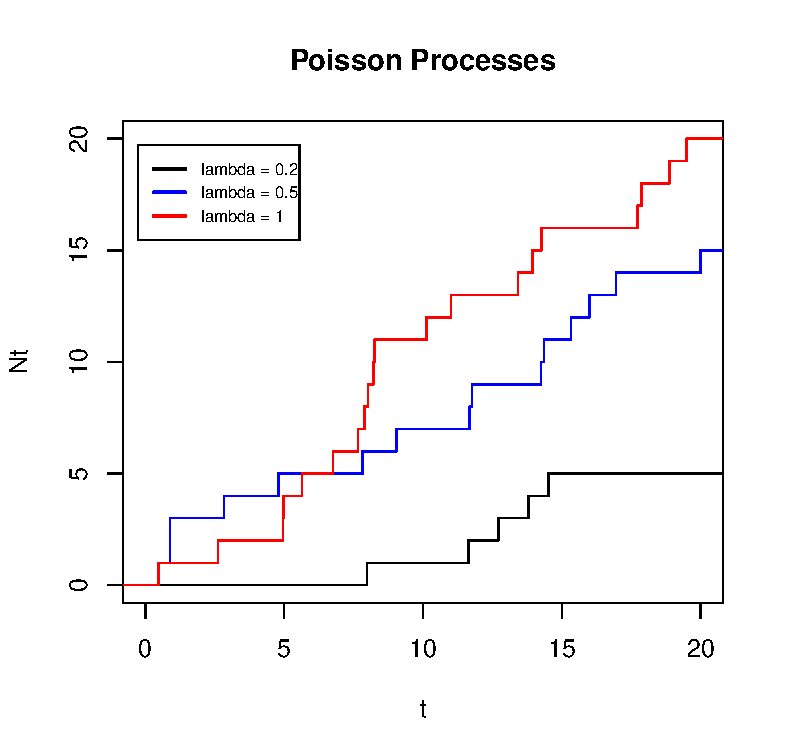
\includegraphics[width=\linewidth]{Images/poisson_process.pdf}
		\caption{Poisson processes.}
		\label{fig:pois}
	\end{subfigure}%
	\begin{subfigure}{.5\textwidth}
		\centering
		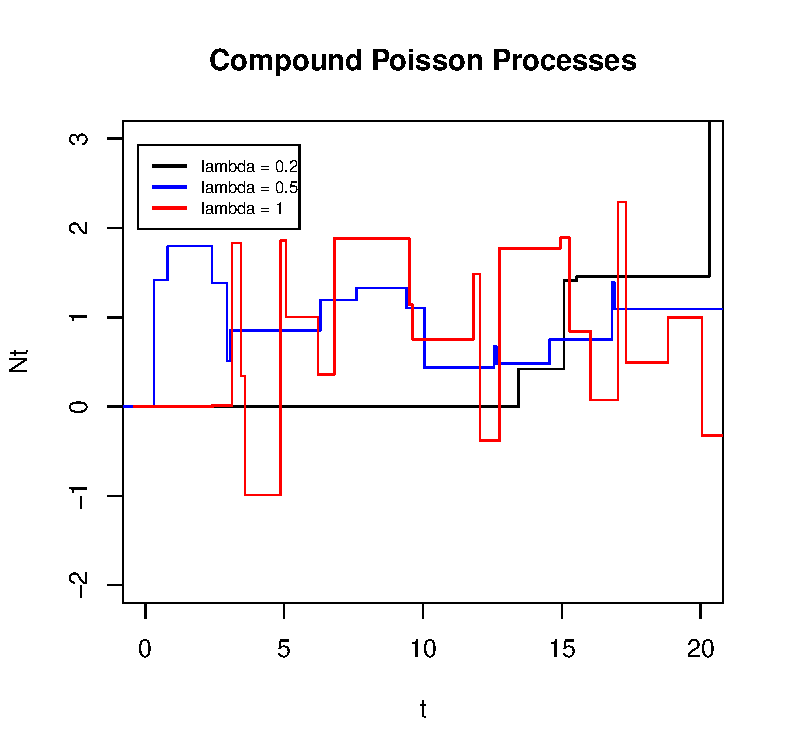
\includegraphics[width=\linewidth]{Images/compound_poisson_process.pdf}
		\caption{Compound with Gaussian jumps.}
		%$\mathcal{N}(1,1)$
		\label{fig:compound_pois}
	\end{subfigure}
	\caption{Poisson processes and compound Poisson processes with different $\lambda$.}
	\label{fig:pois_process}
\end{figure}

When working with jump diffusion process, it is often the case that there is no explicit formula for its density, thus usually we resort to characteristic functions. The characteristic function of $N_t$ is given by 
\begin{equation}
\label{eq:pois_chf}
	\phi_{N_t}(u)=e^{\lambda t (e^{iu}-1)}
\end{equation}

The computations to get \ref{eq:pois_chf} from \ref{eq:pois_pdf} are carried out in Appendix \ref{app:A}. 

\bigskip
For financial applications, it is of little interest to have a process with a single possible jump size. The \textit{compound} Poisson processes are a generalization of Poisson processes  where  the jump sizes can have an arbitrary distribution. More precisely, consider a Poisson process $N_t$ with parameter $\lambda$ and a sequence of i.i.d\footnote{i.i.d stands for independent and identically distributed.} variables ${Y_i}_{i\geq 1}$ with law $f_Y(y)$. Then the process defined by
\begin{equation}
	X_t = \sum_{n=1}^{N_t} Y_i
\end{equation}
is a compound Poisson process. Examples of this kind of process are plotted in Figure \cref{fig:compound_pois}.

As before, we developed the computations to obtain an expression for the characteristic function of $X_t$ in Appendix \ref{app:A}. The resulting expression depends on the distribution of $Y$, specifically from its characteristic function $\phi_Y(u)$:

\begin{equation}
	\phi_{X_t}(u) = e^{\lambda t (\phi_Y(u)-1)}
\end{equation}

Both in Merton's and in the Heston's models there will be a jump component driven by a compound Poisson process with Gaussian jump sizes, as we will see in the following paragraphs.

\subsection{CIR Process}
The CIR process was introduced in \cite{CIR85} in 1985 by Cox, Ingersoll and Ross (hence the name CIR) as a generalization of a Vasicek process to model the mean reverting dynamics of interest rates.
Following their notation, the differential equation for the  evolution of the rate is given by:
\begin{equation}
\label{eq:cir}
	dr_t = \kappa(\theta - r_t) dt + \sigma \sqrt{r_t}dW_t
\end{equation}
where we have three parameters that characterize it: $\theta$ is the \textit{long-term value} of the rate, the asymptotic level which it tends to settle at in the long run;$\kappa$ is the \textit{mean-reversion rate}, the speed at which the rate is pulled back to the $\theta$ value; finally $\sigma$ accounts for the \textit{volatility} of the stochastic component.
When $\kappa,\theta >0$, equation (\ref{eq:cir}) represents a first order mean-reverting auto-regressive process. Moreover, thanks to \textbf{*****add citation*******}, we know that the process will not hit zero if the following condition is satisfied:
\begin{equation}
	2\kappa\theta > \sigma^2
\end{equation}
This condition is usually referred to as \textit{Feller} condition, from the author of the cited paper in which this result was first presented.

An example of a CIR process is shown in Figure (\ref{fig:cir_proc}), where the mean-reverting effect is  clearly visible.

\begin{figure}
	\centering
	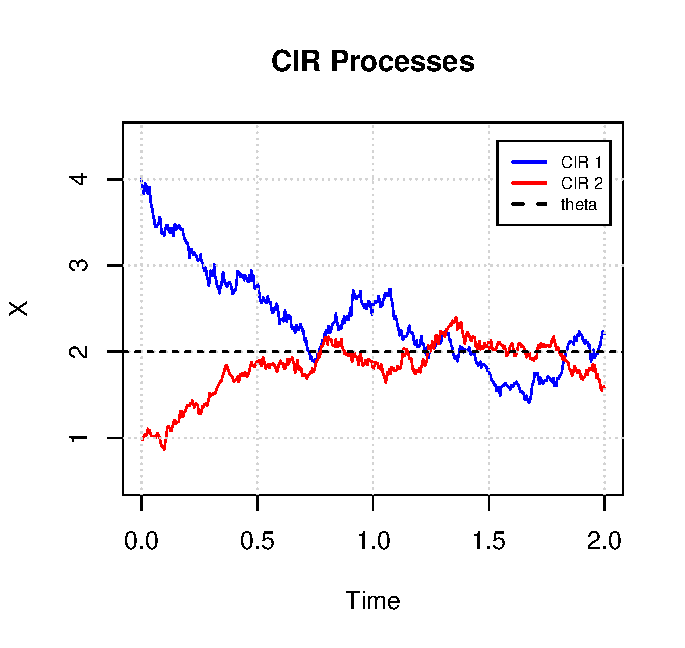
\includegraphics[width=0.6\textwidth]{Images/cir_process.pdf}
	\caption{Two trajectories of the same CIR process: $dr_t = 3(2 - r_t) dt + 0.5 \sqrt{r_t}dW_t$ with different starting point. We can see the mean-reverting effect that attracts both trajectories to the value $\theta=2$. }
	\label{fig:cir_proc}
\end{figure}

When modelling interest rate in continuous time, having $r_t$ hit zero is not an issue since when $r_t=0$ equation (\ref{eq:cir}) reduces to $dr_t = \kappa\theta dt$ which immediately brings the level back to positive values and hence the square root in the dynamics never loses meaning. Conversely, considering a \textit{discretized} version of (\ref{eq:cir}), as is the case in a simulation framework, one needs to pay attention on how he models the increments since a simple Euler discretization scheme may cause $r_t$ to reach \textit{negative} values\footnote{This model was introduced having in mind the certainty that interest rates could never be negative, hence the introduction of a square root in the dynamics. Given recent years interest rates levels, this in no more the case.} and invalidate the whole model representation.

The non negativity of the CIR process will become fundamental when we introduce Heston and Bates SV models, where the (stochastic) variance of the process driving the asset price will be model as a CIR process.

\textcolor{red}{******AGGIUNGERE DISTRIBUZIONE DI rt e di r-inf (gamma)******}

\bigskip
\section{Merton Model}

 ******maybe add some words right here ********
%%% ORIGINAL MODEL
\subsection{Original Univariate Model}
The first jump diffusion model was originally introduced in \cite{MERTON1976} in order to account for the leptokurtic distribution of real market returns and to model sudden falls (or rises) in prices due to the arrival of new information.
The asset price dynamics $S_t$ is modelled as a GBM to which a jump component driven by a compound Poisson process is added:

\begin{equation}
\label{merton_model}
\frac{dS_t}{S_t} = \alpha dt + \sigma dW_t  + (Y_t-1)dN
\end{equation}

where $\alpha$ and $\sigma$ are respectively the drift and the diffusion of the continuous part, $Y_t$ is a process modelling the intensity of the jumps and $N(t)$ is the Poisson process driving the arrival of the jumps and has parameter $\lambda$.

We can rewrite (\ref{merton_model}) in terms of the log-returns $X_t = log(S_t)$ and obtain, following the computations in \cite{MARTIN2007} and using theory from \cite{TANKOV2015}:
\begin{equation}
dX_t = (\alpha - \frac{\sigma^2}{2})dt + \sigma dW_t + \log (Y_t)
\end{equation}

that has as solution:
\begin{equation}
\label{merton_returns}
X_t =X_0 +  \mu t + \sigma W_t + \sum_{k=1}^{N(t)} \eta_k
\end{equation}

where $X_0$ is the initial value of the log-returns, $\eta_k= \log(Y_k) = \log(Y_{t_k})$ and $t_k$ is the time when the $k^{th}$ Poisson shock from $N(t)$ happens. We use $\mu = \alpha - \frac{\sigma^2}{2} $ for ease of notation throughout the paper.
Following \cite{MERTON1976}, we take $\eta_k$ \textit{i.i.d.} (independent and identically distributed) and Gaussian, in particular $\eta \sim \mathcal{N}(\theta, \delta^2)$.
Another choice for the distribution of $\eta$ is given in \cite{KOU2002}. 

%% AGGIUNGERE DENSITA' NEL caso generale [0,T] ?

It is often useful when dealing with market data that are by nature discrete, to consider a \textit{discretized} version of (\ref{merton_returns}) in which the values are sampled at intervals of $\Delta t$ in $[0, T]$. We thus get that for $X_i = \log(\frac{S_{i+1}}{S_i})$:

\begin{equation}
\label{discrete_returns}
X_i =  \mu \Delta t + \sigma \sqrt{\Delta t} \; z +  \sum_{k=1}^{N_{i+1} - N_i} Y_k
\end{equation}

where we denote $X_i = X_{t_i}$, $N_i = N(t_i)$ and $t_i = i \Delta t$ with $i= 0 \dots N$, $t_N = N \Delta t= T$,  $z$ is distributed as a standard Gaussian $ z\sim \mathcal{N}(0,1)$.

The Poisson process $N(t)$ in (\ref{discrete_returns}) is computed at times $t_{i+1}$ and $t_i$ and these quantities are subtracted. Following basic stochastic analysis, one can prove that the resulting value $N_{i+1} - N_i$,  is distributed as a Poisson random variable $N$ of parameter $\lambda \Delta t$.
This allows us to provide an explicit formulation for the transition density of the returns using the theorem of total probability:

\begin{equation}
\label{transitional}
f_{\Delta X} (x) = \sum_{k=0}^{\infty} \mathbb{P}(N = k) f_{\Delta X | N = k}(x) 
\end{equation}

This is an infinite mixture of Gaussian distributions, due to the infinite possible realization of the Poisson variable, and renders the estimation of the model through MLE technique intractable, see \cite{HONORE1998}.
To solve this problem we introduce a first order approximation, as it's been proposed in \cite{BALLTOROUS1983}. Considering small $\Delta t$, so that also $\lambda \Delta t $ is small, we obtain that the only relevant terms in (\ref{transitional}) are the one for $ k = 0, 1$.
The formula for the transition density becomes:
\begin{equation*}
f_{\Delta X} (x) = \mathbb{P}(N = 0) f_{\Delta X | N = 0}(x) + \mathbb{P}(N = 1) f_{\Delta X | N = 1}(x)
\end{equation*}
expressing it explicitly:
\begin{equation}
f_{\Delta X} (x) = (1 - \lambda \Delta t) \;f_{\mathcal{N}}(x ; \mu, \sigma^2) + (\lambda \Delta t)\; f_{\mathcal{N}}(x ; \mu + \theta, \sigma^2+\delta^2)
\end{equation}
where $f_{\mathcal{N}}(x ; \mu, \sigma^2)$ is the density of a Gaussian with parameters $\mathcal{N}(\mu, \sigma^2)$.


%%% MULTIVARIATE MODEL
\subsection{Multivariate Model}
Starting from the univariate model introduced in \cite{MERTON1976}, we developed a generalization to $n$ assets including only idiosyncratic jumps:

\begin{equation}
\frac{dS_t^{(j)}}{S_t^{(j)}} = \alpha_j dt + \sigma_j dW_t^{(j)} + (Y^{(j)}_t -1) dN^{(j)}_t
\end{equation}

where $\mathbf{S}_t$ are the prices of the assets, $j = 1 ... n$ represents the asset, $\alpha_j$ are the drifts, $\sigma_j$ are the diffusion coefficients, $W^{(j)}_t$ are the components of an $n$-dimensional Wiener process $ \mathbf{W}_t$ with $dW^{(j)}dW^{(i)}=\rho_{j,i}$, $\eta_j$ represent the intensities of the jumps and are distributed as Gaussian: $\eta_j \sim \mathcal{N}(\theta_j , \delta_j^2)$. Finally, $N^{(j)}(t)$ are Poisson processes with parameters $\lambda_j$, which are independent of $\mathbf{W}_t$ and of one another. 

In order to calibrate the parameters to the value of the market log-returns, we used a Maximum Likelihood approach. We thus maximize:
\begin{equation}
\mathcal{L}(\psi | \Delta \mathbf{x}_{t_1},\Delta \mathbf{x}_{t_2},\dots,\Delta \mathbf{x}_{t_N}) = \sum_{i=1}^{N} f_{\Delta \mathbf{X}}(\Delta\mathbf{x}_{t_i} | \psi)
\end{equation}

where $\psi = \{ \{\mu_j\},\{\sigma_j\},\{\rho_{i,j}\},\{\theta_j\},\{\delta\}_j,\{\lambda_j\} \}$ are the model parameters, $f_{\Delta \mathbf{X}}$ is the transitional density of the log-returns which is computed approximately using the theorem of total probability.
For a full insight on the model and the calibration procedure, please refer to the *APPENDIX LINK*

\bigskip

\section{Heston Model}

The Heston model was presented in 1993 in \cite{HESTON93} as a new framework to model stochastic volatility in the asset price dynamics, which allows to better fit the skewness and kurtosis of the log-return distribution.

\subsection{Univariate Heston Model}
The Heston model belongs to the family of SD processes, generalizations of B\&S model in which the volatility is no more constant but is itself  stochastic.
\textcolor{red}{***add examples?***}
%Example of SD processes are Heston, CEV, sabr, 3/2 model....

Starting with a GBM as in the B\&S framework, we obtain the dynamics of the price process simply by allowing the volatility in (\ref{eq:GBM}) to evolve over time and specifying how this evolution takes place.
In particular, the dynamics of the \textit{instantaneous} variance $V_t = \sigma_t^2$ for the Heston model is described by a CIR process :
\begin{equation}
	\frac{dS_t}{S_t} = \mu dt +\sqrt{ V_t} dW_t^S
\end{equation}
\begin{equation}
	dV_t = \kappa (\theta - V_t) dt + \sigma_V \sqrt{V_t} dW_t^V
\end{equation}

where $\mu$ represents the drift in the asset prices, $\kappa>0$ and $\theta>0$ are respectively the \textit{mean-reversion} rate  and the long-run level for the $V_t$ process, $\sigma_V>0$ is often referred to as the \textit{volatility of volatility} parameter, in short vol-of-vol.
The two brownian motions $W_t^S$ and $W_t^V$ are correlated with correlation coefficient equal to $\rho$.
The variance process is always strictly positive if the Feller condition $2\kappa\theta > \sigma_V$ is satisfied.

Let us now consider the dynamics of the log-return $x_t = \log (S_t)$, as we did in the Merton case. 
Unfortunately, given the increased complexity of the model due to the SV part, an explicit formula for the density of the log-return is not available and it has to be computed from the Fourier inversion of the characteristic function:
\begin{equation}
\label{eq:chf_inversion}
f_{x_t}(x) = \frac{1}{2\pi}\int_{-\infty}^{+\infty} \phi_{x_t}(i u) e^{i u x} du
\end{equation}

In (\ref{eq:chf_inversion}) we omitted the dependence of $f_{x_t}(x)$ and $\phi_{x_t}(u)$ on model parameters and on the initial values of the log-returns $x_0$ and of the variance process $V_0$. 

\bigskip

To derive the expression of the characteristic function $\phi_{x_t}(u)$, one has to solve a couple of \textit{Fokker-Planck} partial differential equation as is shown in the Appendix of the reference paper by Heston \cite{HESTON93}. This procedure is beyond the scope of this thesis and thus we will only report the final result, which is a log-affine equation on the information at time $t = 0$:

\begin{subequations}
\begin{align}
	\phi_{x_t}(u| x_0, V_0) &= \exp\{A(t,u) + B(t,u) x_0 + C(t,u) V_0\}\nonumber \\
	A(t,u) &= \mu u i t +  \frac{\kappa\theta}{\sigma_V^2} \bigg( (\kappa - \rho\sigma_V u i +d)t - 2 \log\Big[  \frac{1-ge^{dt}}{1-g} \Big] \bigg)\\
	B(t,u) &= i u \\
	C(t,u)&= \frac{\kappa - \rho\sigma_V u i +d}{\sigma_V^2} \:\Big[\frac{1-e^{dt}}{1+ge^{dt}}\Big]
\end{align}
\end{subequations} 
where :
\begin{equation*}
\begin{split}
d&=\sqrt{(\rho \sigma_V u i - \kappa)^2 + \sigma_V^2(u i + u^2)}\\
g&= \frac{\kappa - \rho\sigma_V u i + d}{\kappa - \rho\sigma_V u i - d}
\end{split}
\end{equation*} 



This formulation is the one proposed by Heston in his original paper \cite{HESTON93} but it is shown in \cite{HESTONTRAP}  that it has numerical issues when  pricing Vanilla options using Fourier methods. We will not be pricing any instrument, however we may incur in the same errors when calibrating our model through the techniques explained in Chapter \ref{chpr:calibration}. For this reason, we will be using the alternative formulation presented in \cite{HESTONTRAP}:



%\begin{IEEEeqnarray*}{rCL}
%	\phi_{x_t}(u| x_0, V_0) &=& \exp\{A(t,u) + B(t,u) x_0 + C(t,u) V_0\} \IEEEyesnumber\\
%	A(t,u) &= &\mu u i t +  \frac{\kappa\theta}{\sigma_V^2} \bigg( (\kappa - \rho\sigma_V u i +d)t - 2 \log\Big[  \frac{1-ge^{+dt}}{1-g} \Big] \bigg) \IEEEyessubnumber*\\
%	B(t,u) &= &i u \\
%	C(t,u) &=& \frac{\kappa - \rho\sigma_V u i +d}{\sigma_V^2} \:\Big[\frac{1-ge^{+dt}}{1+g}\Big]\\
%\end{IEEEeqnarray*}

\begin{equation}
% heston trap solution
\begin{split}
\phi_{x_t}^*(u| x_0, V_0) &= \exp\{A(t,u) + B(t,u) x_0 + C(t,u) V_0\}\\
A(t,u) &= \mu u i t +  \frac{\kappa\theta}{\sigma_V^2} \bigg( (\kappa - \rho\sigma_V u i - d)t - 2 \log\Big[  \frac{1-g^*e^{-dt}}{1-g^*} \Big] \bigg)\\
B(t,u) &= i u \\
C(t,u)&= \frac{\kappa - \rho\sigma_V u i - d}{\sigma_V^2} \:\Big[\frac{1-e^{-dt}}{1-g^*e^{-dt}}\Big]
\end{split}
\end{equation} 
where :
\begin{equation*}
\begin{split}
d&=\sqrt{(\rho \sigma_V u i - \kappa)^2 + \sigma_V^2(u i + u^2)}\\
g^*&= \frac{\kappa - \rho\sigma_V u i - d}{\kappa - \rho\sigma_V u i + d} = \frac{1}{g}
\end{split}
\end{equation*} 

The only difference is that the signs of the $d$ terms are all flipped: the origin of the two representations for the characteristic function lies in the fact that the complex root $d$ has two possible values and the second value is exactly minus the first value.
A uniform choice between the two possibilities cannot be made over all the complex plane to obtain a continuous function due to the presence of a branch cut in the graph of $\sqrt{z}$. Selecting the sign of $d$ as in $\phi_{x_t}^*$ and $g^*$ avoids the discontinuity affecting our future computations.

\bigskip


Our characteristic function still depends on the initial values $x_0$ and  $V_0$ and is thus often called \textit{conditional} characteristic function on $x_0$ and $V_0$.
We can easily remove the dependence on $x_0$ by considering the distribution of incremental returns, namely $\Delta x_t = \log (S_t / S_0) = x_t - x_0$
%, but as for $V_0$, we will need to do some more work.

Applying the definition of characteristic function:
\begin{equation*}
	\begin{split}
	\phi_{\Delta x_t}(u) &= \mathbb{E}\big[e^{i u \Delta x_t} \big] \\
	&=  \mathbb{E}\big[e^{i u ( x_t - x_0)}\big]\\
	&= \mathbb{E}\big[e^{i u x_t}\big] e^{-i u x_0}\\
	&= \phi_{x_t}(u) e^{-i u x_0}\\
	&= \exp\{A(t,u) + (B(t,u) - iu) x_0 + C(t,u) V_0\}
	\end{split}
\end{equation*}

and since $B(t,u)  = i u$, the second term in the exponential is equal to zero and we are left with:
\begin{equation}
\label{eq:chf_V0}
\phi_{\Delta x_t}(u) =  \exp\{A(t,u) + C(t,u) V_0\}
\end{equation}




This equation is however still dependent on the initial value of the variance process. In a simulation framework, this would not be an issue, since we can define the level of $V_0$ ourselves and then generate all the different scenarios. However, if we need to calibrate the model parameters from asset prices, the market data for the variance process are not available. We will address more in depth different ways to solve this problem later on in Chapter \ref{chpr:calibration}. As for now, we show that we can obtain an \textit{unconditional} expression for the characteristic function of a Heston process by approximating the distribution of $V_t$ with its long-run distribution.




\textcolor{red}{\textbf{*** add unconditional chf ***}}
\section{Bates Model}


